\section{Callbacks}
Javascript ist eine ereignisgesteuerte Programmiersprache. Das bedeutet, anstatt auf blockierenden Code zu warten, führt Javascript Operationen weiter aus und reagiert wenn die Aktion fertig ist. Um sicherzustellen, dass Javascript abhängige Funktionen erst nach der Fertigstellung von asynchronen Operationen ausführt, wurde das Prinzip der \textbf{Callbacks} eingeführt.

\subsection{Funktionsweise}

Sowohl in Javascript als auch in Typescript sind Funktionen als Erste-Klasse-Objekte zu sehen. Aus diesem Grund ist es Möglich sie an Variablen zu binden oder als Argumente in anderen Funktionen oder als Rückgabewert zu übergeben. Diese übergebenen Funktionen heißen Callbacks.\\

\noindent
Callbacks, auch Rückruffunktionen genannt, bildet das Kernkonzept der funktionalen Programmierung in Javascript.\cite{callbacks-intro} In der funktionalen Programmierung sind Funktionen als Werte zu betrachten. Der Code besteht aus kleineren Funktionen, die in höher geordneten Funktionen eingesetzt oder miteinander kombiniert werden können (Komposition). Dadurch ist der Code wiederverwendbar und weniger fehleranfällig. Javascript bietet mit Arrays die Möglichkeit Callbacks sinnvoll einzusetzen. Vor dem Ausführen des Beispiels muss folgend konfiguriert werden:

\begin{center}
    async-patterns$\,\to\,$ webpack.config.js
\end{center}

\begin{figure}[H]
\begin{lstlisting}[basicstyle=\small]
module.exports = {
    mode: 'development',
    entry: './src/modules/callbacks/introduction.ts',
    ...
}
\end{lstlisting}
\end{figure}

\begin{figure}[H]
\begin{lstlisting}[basicstyle=\small]
const numbers: number[] = [1, 2, 3, 4, 5, 6];

function isEven(x): boolean { 
  return x % 2 === 0; 
}

const evenNumbers = numbers.filter(isEven);
console.log(evenNumbers) // 2 4 6
\end{lstlisting}
\caption{Die Funktion filter() gibt ein neues Array zurück.}
\end{figure}

\noindent
Die Methode filter() nimmt Elemente einer Liste heraus, basierend einer Funktion die, die Filterkonditionen bestimmt. Dabei wird zuerst, dass Element aus der Liste entnommen und dann die Kondition geprüft. Da Funktionen als Argument anderer Funktionen übergeben werden, ist es Möglich diese \glqq{}später\grqq{} innerhalb des Funktionsrumpfes aufzurufen \textit{(\glqq{}Call back\grqq{})}. Wenn also eine Funktion als Parameter übergeben wird, wird diese nicht sofort ausgeführt. Eine Funktion die ein Callback als Argument annimmt, wird auch höherrangige Funktion \textit{(Higher order function)} genannt.\cite{callbacks-example} Möchte man das Filtern klassisch implementieren, dann würde der Code im Vergleich dazu so aussehen:

\begin{figure}[H]
\begin{lstlisting}[basicstyle=\small]
const newArr = [];

for (let i = 0; i < numbers.length; i++) {
    if (numbers[i] % 2 === 0) {
        newArr.push(numbers[i]);
    }
}

console.log(newArr);
\end{lstlisting}
\end{figure}

\noindent
Wie man nun sehen kann, ist man mit dieser Umsetzung an externe Variablen gebunden. Diese könnte im Verlauf des Codes eventuell überschrieben werden. Das heißt der unten ausgeführte Code ist abhängig vom Status des Arrays. Dies führt zu einer erhöhten Fehleranfälligkeit. Wenn man nun alle ungeraden Zahlen herausfiltern möchte, müsste man ein neues Array mit einer neuen Schleife erstellen. In diesem Fall wird keine Möglichkeit der Wiederverwendbarkeit gewährleistet.

\subsection{Asynchrone Verarbeitung}

Ein Ansatz der asynchronen Verarbeitung ist die Nutzung von Funktionen die eine Funktion als Argument annimmt und erst dann diese Aufrufen, wenn eine blockierende Aktion fertig ausgeführt wurde. Dieses Verhalten ist nützlich wenn der Browser von bestimmten, zeitintensiven Aktionen abhängig ist. Man kann ein synchrones und asynchrones Programmiermodel mit einem kleinem Beispiel vergleichen: Eine Anwendung die zwei Ressourcen aus einem Netzwerk anfragt und die Ergebnisse miteinander kombiniert. In einer synchronen Umgebung würde man dies mit einem Funktionsaufruf nach dem anderen bewältigen. Das hat den Nachteil, dass die zweite Funktion erst dann ausführt, wenn die erste fertig ist. Die Gesamtzeit der Ausführung ist die Summe der Antwortzeiten der beiden Anfragen. Die Lösung dafür ist ein synchrones Programmverhalten mit mehrere kontrollierten Threads. Ein Thread ist ein Ausführungsstrang, der seine eigene Zeitleiste besitzt und innerhalb dieser Operationen ausführt. Ein zweiter Thread könnte zum selben Zeitpunkt die Funktion aufrufen und wenn beide Threads das Ergebnis geliefert bekommen resynchronisieren sie sich und kombinieren ihre Ergebnisse. Im folgenden Diagramm repräsentieren die blauen Linien die Zeit, in der das Programm ausführt und die roten Linien repräsentieren die Zeit, in der auf die Antwort gewartet wird.\cite{asynchronitaet}

\begin{center}
\begin{figure}[H]
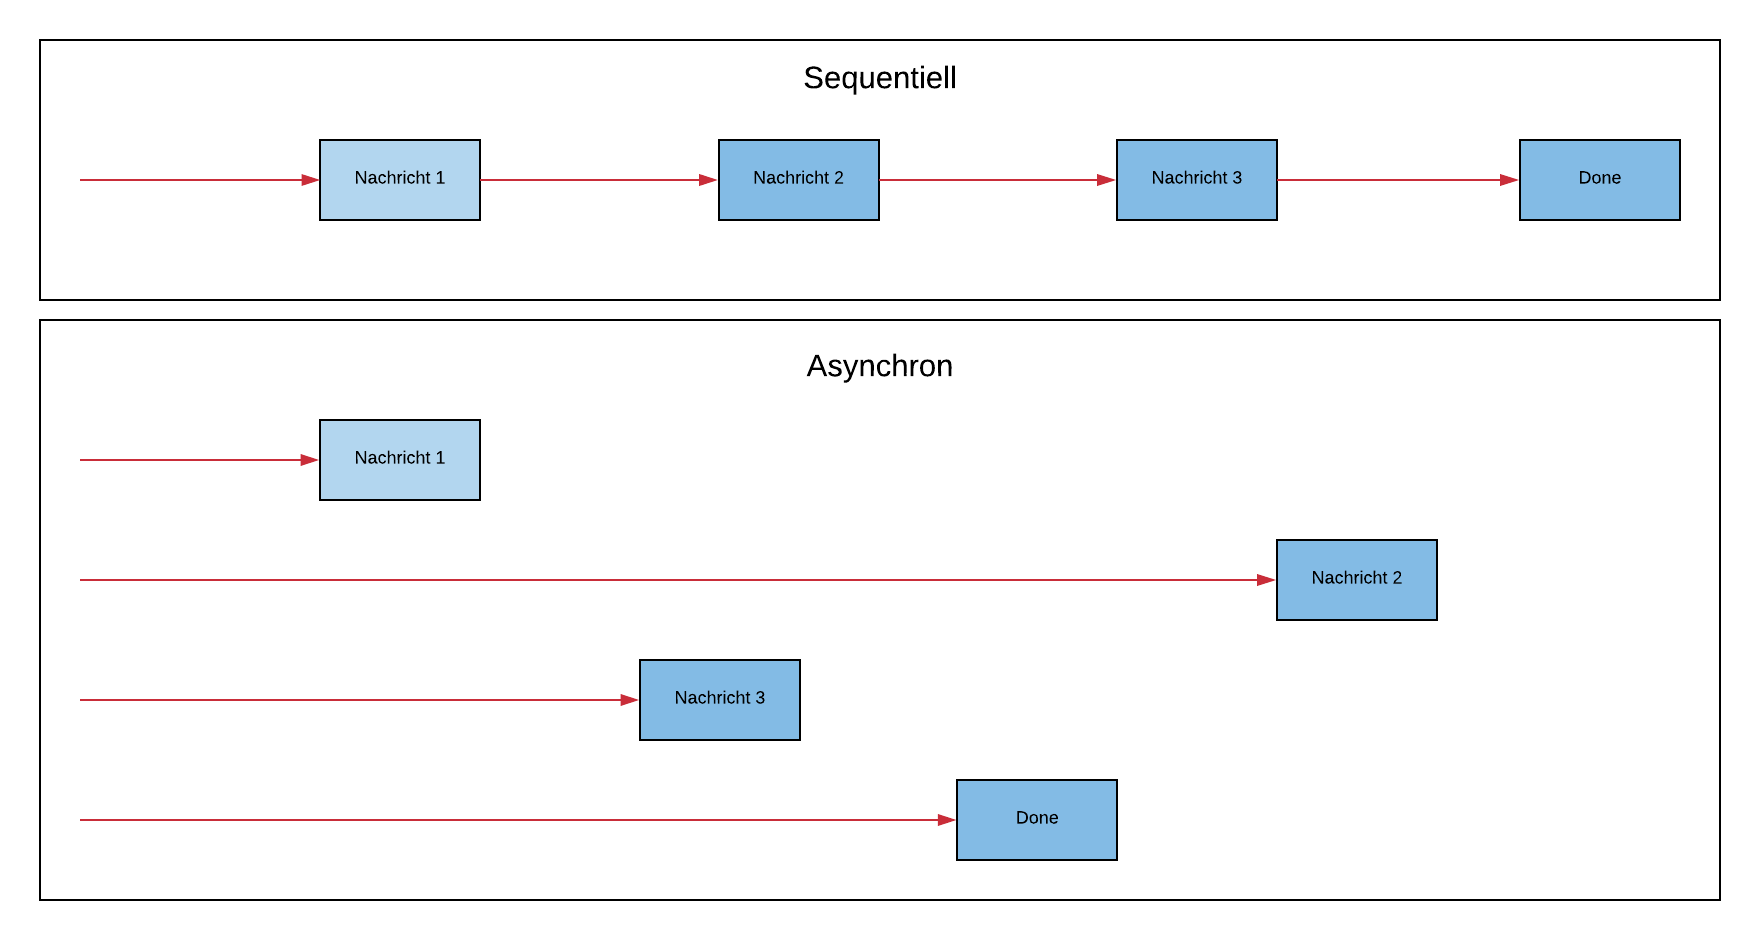
\includegraphics[width=12cm]{synchron-vs-asynchron-diagram}
\end{figure}
\end{center}

\noindent
Im synchronen Modell ist die Zeit der Netzwerkanfrage ein Teil der Zeitleiste. Im asynchronen Modell hingegen führt das Starten einer asynchronen Operation zu einer neuen Zeitleiste. Zusammenfassend kann man also sagen, dass in dem synchronen Modell implizit auf die Aktionen gewartet wird, und in dem asynchronen Modell explizit.

\subsection{Beispiel}
In den Kapitel Callbacks, Promises und Async await wird das gleiche Beispiel, in drei verschiedenen Ausprägungen angewendet und gegenübergestellt. Mit der REST-Api \textbf{JSONPlaceholder} wird ein Endpunkt für die Datenabfrage definiert. Hierbei handelt es sich um eine Open Source Endstelle die Beispieldaten für das Prototyping oder zum Testen zur Verfügung stellt. Je nach Anwendungsfall werden verschiedene Ausführungen von Anfragen an diese Endstelle geführt, um die Code-Beispiele so praxisnah wie Möglich zu halten.\\

\noindent
Das folgende Beispiel richtet sich nach dem funktionalen Programmierparadigma, da durch die Nutzungen von \textbf{puren Funktionen}, das Callback-Prinzip besser zur Geltung kommt. Eine pure Funktion, ist eine Funktion, die beim selben Input jedes mal das gleiche Output wiedergibt. Zu erwähnen ist jedoch, dass das Prinzip der Callbacks auch im objektorientiertem Schema umgesetzt werden kann. Für das Beispiel sollte ../callbacks/stories.ts als Eingangsdatei definiert werden.

\begin{figure}[H]
\begin{lstlisting}[basicstyle=\small]
function makeRequest(url, onSuccess, onFailure?): void {
    const req = new XMLHttpRequest();
    req.open('GET', url);

    req.onload = () => {
        if (req.status === 200) {
            fakeLatency(() => onSuccess(JSON.parse(req.response));
        }
    };

    req.onerror = () => onFailure(Error('Network Error'));

    req.send();
}

function fakeLatency(callback): void {
    setTimeout(callback, 3000 * Math.random());
}

function baseUrl(): string {
    return 'https://jsonplaceholder.typicode.com/posts/';
}

function getAllChapters(onSuccess, onFailure?): void {
    makeRequest(baseUrl(), onSuccess, onFailure);
}

function getChapter(chapter, onSuccess, onFailure?): void {
    makeRequest(baseUrl() + chapter.toString(), onSuccess, onFailure);
}
\end{lstlisting}
\end{figure}

\begin{figure}[H]
\begin{lstlisting}[basicstyle=\small]
function createElm(innerHTML): HTMLElement {
    const div = document.createElement('div');
    div.innerHTML = innerHTML;
    document.body.appendChild(div);
    return div;
}

function spawn(content: any): void {
    if (content instanceof Array === false) {
        content = [content];
    }

    content.forEach(elm => {
        const snippet = document.createElement('div');
        snippet.innerHTML = '<h1>${elm.title}</h1>
                             <div>
                                <i>${elm.id}</i>
                             </div>
                             <p>${elm.body}.</p>';

        document.body.insertBefore(snippet, loadingIcon);
    });
}

function catchError(err) {
     createElm('Ooops! Error Occurred! ${err}');
}

function displayFinished(): void {
    loadingIcon.style.display = 'none';
    createElm('All done!');
}

const loadingIcon = createElm('<svg>..</svg>');
\end{lstlisting}
\end{figure}

\noindent
Dabei sind die wichtigsten Funktionen makeRequest(), getAllChapters(), getChapter() und spawn(). MakeRequest() führt eine Http-Anfrage gegen einen definierten Endpunkt aus. Wenn der Status der Antwort 200 beträgt, wird im Success-Callback vorangeschreitet. Bei einem Fehler wird der Error-Callback aufgerufen. Sowohl getAllChapter() als auch getChapter() führen makeRequest() aus, mit der Möglichkeit im Erfolgs- und im Fehlerfall der Anfrage eine Aktion auszuführen. Spawn() nimmt ein Argument entgegen und lädt diesen in die DOM. Sollte ein Anwendungsfall sein, alle Kapitel der API anzufragen und bei Ankunft der Daten anzuzeigen, würde dies wie folgt aussehen:

\begin{figure}[H]
\begin{lstlisting}[basicstyle=\small]
getAllChapters(function(response) {
    spawn(response);
    displayFinished();
});
\end{lstlisting}
\end{figure}

\noindent
In diesem Fall wird spawn() erst aufgerufen, wenn eine Antwort vom Endpunkt ankommt. Um multiple asynchrone Operationen nacheinander auszuführen, müssen Funktionen ineinandergeschachtelt werden. So wird die Ausführung sequentiell fortgesetzt. Als Beispiel wird Kapitel eins bis drei chronologisch aufgerufen:

\begin{figure}[H]
\begin{lstlisting}[basicstyle=\small]
getChapter(1, function(response1) { // (*)
    spawn(response1);
    getChapter(2, function(response2) { // (**)
        spawn(response2);
        getChapter(3, function(response3) { // (***)
            spawn(response3);
            displayFinished();
        });
    });
});
\end{lstlisting}
\end{figure}

\noindent
Auffallend in diesem Beispiel ist der Grad der Einrückung, der mit jeder weiteren asynchronen Operationen steigt. Ein neuer Thread entsteht schon beim Aufruf von getChapter(1). Alle weiteren asynchronen Operationen sind voneinander abhängig und bleiben innerhalb der selben Zeitleiste. Asynchronität ist ansteckend. Eine Funktion, die zur asynchronen Verarbeitung ein Callback nutzt, operiert selbst asynchron. Wenn nun ein Großteil eines Programms aus ineinandergeschachtelten Funktionen besteht, kann diese Struktur zur erhöhten Fehleranfälligkeit führen. Dank der der sechsten Ecmascript Version ist es auch Möglich Pfeil-Funktionen in Javascript zu nutzen. Diese sind syntaktisch kürzer als anonyme Funktionen. Wenn nun die fehlgeschlagenen Callbacks zusätzlich verarbeitet werden sollen, dann sieht der Code so aus:

\begin{figure}[H]
\begin{lstlisting}[basicstyle=\small]
getChapter(1, response1 => { // (*)
    spawn(response1);
    getChapter(2, response2 => { // (**)
        spawn(response2);
        getChapter(3, response3 => { // (***)
            spawn(response3);
            displayFinished();
        }, err3 => catchError(err3)); // (***)
    }, err2 => catchError(err2)); // (**)
}, err1 => catchError(err1)); // (*)
\end{lstlisting}
\caption{In der Praxis sollte für eine asynchrone Operation wie z.B. ein Http-Aufruf der Fehlerfall immer abgedeckt sein.}
\end{figure}

\noindent
Es bildet sich eine Verzweigung, die sich immer weiter nach rechts ausbreitet. Zudem ist es auf dem ersten Blick schwer zu erkennen welcher Error-Callback zu welchem Kapitelaufruf gehört. Wie man nun sehen kann, ist es möglich mit Callbacks asynchron Daten zu verarbeiten. Bei mehreren abhängigen asynchronen Prozessen müssen Callbacks ineinandergeschachtelt werden. Mehrere Level von geschachtelten Callbacks führen zu einer schwer nachvollziehbaren Code-Struktur. Deshalb wird der Code in Abbildung 6 auch als \glqq{}Callback-Hell\grqq{} bezeichnet. Um aus der Callback-Hell zu entkommen, ebnete Ecmascript 6 den Weg der nativen Nutzung von \textbf{Promises}.



